
本书的大部分内容将展示如何为用户准备CMake项目,要彻底了解用户在不同场景下如何与CMake交互。将允许测试项目文件,并确保它们工作正常。

CMake是一个工具集,由五个可执行程序组成:

\begin{itemize}
\item 
cmake: 配置、生成和构建项目的主要可执行文件。

\item 
ctest: 用于运行和报告测试结果的测试驱动程序。

\item 
cpack: 用来生成安装程序和源包的打包程序。

\item 
cmake-gui: cmake的图形界面。

\item 
ccmake: cmake基于控制台的图形界面。
\end{itemize}

\subsubsubsection{1.4.1\hspace{0.2cm}CMake}

提供了一些操作模式(也称为动作):

\begin{itemize}
\item 
生成项目构建系统

\item 
构建项目

\item 
安装项目

\item 
运行脚本

\item 
运行命令行工具

\item 
获得帮助
\end{itemize}

\hspace*{\fill} \\ %插入空行
\noindent
\textbf{生成项目构建系统}

这是构建项目的第一步,关于如何执行CMake构建操作的选项:

\begin{tcblisting}{commandshell={}}
# 生成模式的语法

cmake [<options>] -S <path-to-source> -B <path-to-build>
cmake [<options>] <path-to-source>
cmake [<options>] <path-to-existing-build>
\end{tcblisting}

我们将在接下来的部分中讨论这些选项。现在,让我们集中精力选择正确的命令形式。CMake的重要特性是支持源外构建或在单独目录中生成工件。与GNU Make等工具相比,这确保源目录与构建相关的文件保持分离,并避免不必要的文件污染版本控制系统(VCS)或忽略指令。这就是为什么最好使用生成模式的第一种形式的命令:用-S选项指定源树的路径,然后用-B选项指定生成的构建系统的目录:

\begin{tcblisting}{commandshell={}}
cmake -S ./project -B ./build
\end{tcblisting}

上面的命令将从./project目录中的源代码中在./build目录中生成一个构建系统(如果没有就创建)。

可以跳过其中一个参数,cmake将“猜测”我们打算使用当前目录。跳过这两者将形成内源代码构建,这很麻烦。

\begin{tcolorbox}[colback=red!5!white,colframe=red!75!black,title=不推荐]
不要使用cmake <directory>命令的第二种或第三种形式,因为它会产生一个混乱的内源代码构建(我们将在第3章中学习如何阻止它)。正如语法片段中所示,若<directory>中已经存在先前的构建,则相同的命令的行为不同,将使用到源的缓存路径并从那里重新构建。由于经常使用终端命令历史中运行相同的命令,因此在这里可能会遇到麻烦。使用此方式之前,请检查shell当前是否在正确的目录下。
\end{tcolorbox}

\textbf{示例}

在当前目录中构建,但从一个目录中获取源代码(-S是可选的):

\begin{tcblisting}{commandshell={}}
cmake -S ..
\end{tcblisting}

在./build目录中编译,并使用当前目录中的源代码:

\begin{tcblisting}{commandshell={}}
cmake -B build
\end{tcblisting}

\hspace*{\fill} \\ %插入空行
\noindent
\textbf{生成器的选项}

可以在生成阶段指定一些选项。选择和配置生成器决定了将使用哪个构建工具进行构建,构建文件是什么样子的,以及构建树的结构。
 
CMake确实支持许多平台上的多个原生构建系统,除非你同时安装了几个,否则CMake会正确地选择。选项可以使用CMAKE\_GENERATOR环境变量覆盖,或者直接在命令行上指定生成器:

\begin{tcblisting}{commandshell={}}
cmake -G <generator-name> <path-to-source>
\end{tcblisting}

一些生成器(如Visual Studio)支持更深入的工具集(编译器)和平台(编译器或SDK)规范。此外,各自有覆盖默认值的环境变量:CMAKE\_GENERATOR\_TOOLSET和CMAKE\_GENERATOR\_PLATFORM。也可以直接指定:

\begin{tcblisting}{commandshell={}}
cmake -G <generator-name>
      -T <toolset-spec> -A <platform-name>
      <path-to-source>
\end{tcblisting}

Windows用户通常希望为他们喜欢的IDE生成一个构建系统。在Linux和macOS上,使用Unix Makefiles或Ninja生成器比较常见。

要检查系统上有哪些生成器可用,使用以下命令:

\begin{tcblisting}{commandshell={}}
cmake --help
\end{tcblisting}

帮助信息输出的最后,应该可以看到一个完整的列表:

\begin{tcblisting}{commandshell={}}
# Windows 10上有很多可用的生成器

The following generators are available on this platform:
Visual Studio 16 2019
Visual Studio 15 2017 [arch]
Visual Studio 14 2015 [arch]
Visual Studio 12 2013 [arch]
Visual Studio 11 2012 [arch]
Visual Studio 10 2010 [arch]
Visual Studio 9 2008 [arch]
Borland Makefiles
NMake Makefiles
NMake Makefiles JOM
\end{tcblisting}
\begin{tcblisting}{commandshell={}}
MSYS Makefiles
MinGW Makefiles
Green Hills MULTI
Unix Makefiles
Ninja
Ninja Multi-Config
Watcom Wmake
CodeBlocks - MinGW Makefiles
CodeBlocks - NMake Makefiles
CodeBlocks - NMake Makefiles JOM
CodeBlocks - Ninja
CodeBlocks - Unix Makefiles
CodeLite - MinGW Makefiles
CodeLite - NMake Makefiles
CodeLite - Ninja
CodeLite - Unix Makefiles
Eclipse CDT4 - NMake Makefiles
Eclipse CDT4 - MinGW Makefiles
Eclipse CDT4 - Ninja
Eclipse CDT4 - Unix Makefiles
Kate - MinGW Makefiles
Kate - NMake Makefiles
Kate - Ninja
Kate - Unix Makefiles
Sublime Text 2 - MinGW Makefiles
Sublime Text 2 - NMake Makefiles
Sublime Text 2 - Ninja
Sublime Text 2 - Unix Makefiles
\end{tcblisting}

\hspace*{\fill} \\ %插入空行
\noindent
\textbf{缓存选项}

CMake在配置阶段向系统查询各种信息,这些信息缓存在构建树目录中的CMakeCache.txt中。

可以想到的第一件事是预填充缓存信息:

\begin{tcblisting}{commandshell={}}
cmake -C <initial-cache-script> <path-to-source>
\end{tcblisting}

可以提供到CMake脚本的路径,该脚本(仅)包含set()指令的列表,以指定将用于初始化空构建树的变量。

现有缓存变量的初始化和修改可以用另一种方式完成(例如,创建文件时只设置几个变量有点多)。可以简单地在命令行中设置它们:

\begin{tcblisting}{commandshell={}}
cmake -D <var>[:<type>]=<value> <path-to-source>
\end{tcblisting}

:<type>部分是可选的(用在GUI端),可以使用BOOL、FILEPATH、PATH、STRING或INTERNAL。若省略了类型,将设置为一个已经存在的变量的类型;否则,将设置为UNINITIALIZED。

一个特别重要的变量包含构建的类型:例如,Debug和Release。许多CMake项目将在许多场景下运行,以决定符号信息的冗长程度、调试信息的存在程度,以及所创建工件的优化级别。

对于单配置生成器(如Make和Ninja),需要在配置阶段使用CMAKE\_BUILD\_TYPE变量指定构建类型,并为每种类型的配置生成单独的构建树:Debug、Release、MinSizeRel或RelWithDebInfo。

这有一个例子:

\begin{tcblisting}{commandshell={}}
cmake -S . -B build -D CMAKE_BUILD_TYPE=Release
\end{tcblisting}

注意,多配置生成器是在构建阶段配置的。

可以用-L选项列出缓存变量:

\begin{tcblisting}{commandshell={}}
cmake -L[A][H] <path-to-source>
\end{tcblisting}

这样的列表将包含未标记为ADVANCED的缓存变量,可以通过参数A进行改变。要打印带有变量的帮助消息——需要添加H参数。

使用-D选项手动添加的自定义变量将不可见,除非指定受支持的类型之一。

删除一个或多个变量可以通过以下选项完成:

\begin{tcblisting}{commandshell={}}
cmake -U <globbing_expr> <path-to-source>
\end{tcblisting}

这里,通配符表达式支持*通配符和任何?字符,使用时需要倍加小心。

-U和-D选项都可以重复多次使用。

\hspace*{\fill} \\ %插入空行
\noindent
\textbf{用于调试和跟踪的选项}

CMake可以通过许多选项来运行,这些选项可以让您了解内部发生了什么。要获取关于变量、命令、宏和其他设置的一般信息,运行以下命令:

\begin{tcblisting}{commandshell={}}
cmake --system-information [file]
\end{tcblisting}

可选的file参数允许将输出存储在文件中。在构建树目录中运行,将从日志文件中打印有关缓存变量和构建消息的信息。

项目中,将使用message()报告构建过程的细节,CMake根据当前日志级别(默认情况下是STATUS)过滤这些日志的输出。下面的命令行指定了感兴趣的日志级别:

\begin{tcblisting}{commandshell={}}
cmake --log-level=<level>
\end{tcblisting}

这里的级别可以是其中一个:ERROR、WARNING、NOTICE、STATUS、VERBOSE、DEBUG或TRACE。可以在CMAKE\_MESSAGE\_LOG\_LEVEL缓存变量中永久地保留这个设置。

另一个有趣的选项允许显示每个message()的日志上下文。要调试非常复杂的项目,可以像使用堆栈一样使用CMAKE\_MESSAGE\_CONTEXT变量。当代码进入特定上下文时,可以向堆栈添加描述性名称,并在离开时删除它。通过这样做,消息将用当前的CMAKE\_MESSAGE\_CONTEXT变量装饰:

\begin{tcblisting}{commandshell={}}
[some.context.example] Debug message.
\end{tcblisting}

启用这种日志输出的选项如下:

\begin{tcblisting}{commandshell={}}
cmake --log-context <path-to-source>
\end{tcblisting}

我们将在第2章中更详细地讨论。

若所有这些都失败了——需要使用大型武器——跟踪模式。这将打印每个命令的文件名和调用的确切行号及其参数。可以通过以下方式启用:

\begin{tcblisting}{commandshell={}}
cmake --trace
\end{tcblisting}

\hspace*{\fill} \\ %插入空行
\noindent
\textbf{预置的选项}

用户可以指定许多选项来从您的项目生成构建树。在处理构建树路径、生成器、缓存和环境变量时,很容易混淆或遗漏某些内容。开发人员可以简化用户与项目交互的方式,并提供CMakePresets.json文件,其指定了一些默认值。

要列出所有可用的预设,可以执行以下命令:

\begin{tcblisting}{commandshell={}}
cmake --list-presets
\end{tcblisting}

使用预设的方式如下所示:

\begin{tcblisting}{commandshell={}}
cmake --preset=<preset>
\end{tcblisting}

这些值覆盖系统默认值和环境。与此同时,也可以显式地在命令行上传递的参数所覆盖:

\begin{center}
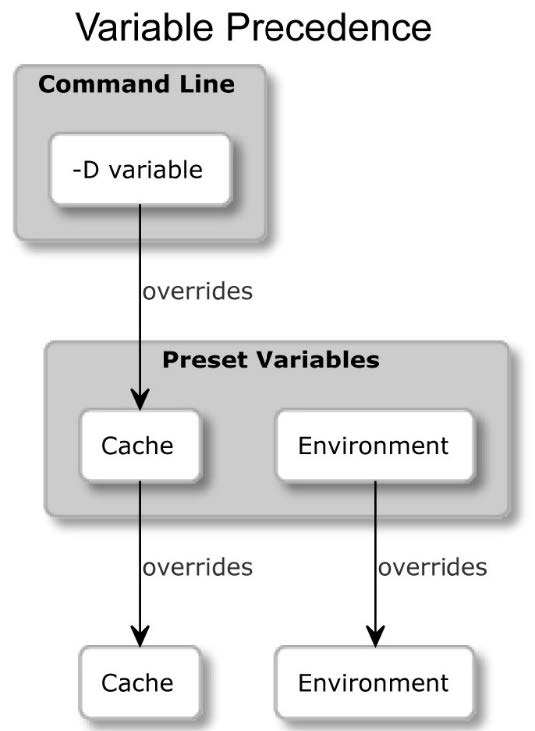
\includegraphics[width=0.5\textwidth]{content/1/chapter1/images/3.jpg}\\
图1.3 预设如何覆盖CMakeCache.txt和系统环境变量
\end{center}

\hspace*{\fill} \\ %插入空行
\noindent
\textbf{构建项目}

生成构建树后,就可以进入下一个阶段:运行构建器工具。CMake不仅知道如何为许多不同的构建器生成输入文件,还可以使用特定于项目参数运行。

\begin{tcolorbox}[colback=red!5!white,colframe=red!75!black,title=不推荐]
许多在线资源建议在生成阶段之后直接运行GNU Make: make。这是Linux和macOS的默认生成器,可以正常工作。但更推荐本节中描述的方法,与生成器无关,并且在所有平台上都得到支持。因此,不需要担心应用程序的每个用户的确切环境。
\end{tcolorbox}

\begin{tcblisting}{commandshell={}}
# 构建模式的语法

cmake --build <dir> [<options>] [-- <build-tool-options>]
\end{tcblisting}

大多数情况下,只要提供最基本的内容就可以获得成功的构建:

\begin{tcblisting}{commandshell={}}
cmake --build <dir>
\end{tcblisting}

CMake需要知道构建树在哪里,与在生成阶段使用-B参数传递的路径相同。

通过提供一些选项,CMake允许指定适用于每个构建器的关键构建参数。若需要为所选的本机构建器提供特殊参数,请在命令末尾-{}-后传递:

\begin{tcblisting}{commandshell={}}
cmake --build <dir> -- <build-tool-options>
\end{tcblisting}

\hspace*{\fill} \\ %插入空行
\noindent
\textbf{并行构建的选项}

默认情况下,许多构建工具将使用多个并发进程并行编译源代码。构建者知道项目的依赖关系,因此可以同时处理满足依赖关系的步骤,从而节省用户的时间。

若是在功能强大的机器上构建(或强制使用单线程构建进行调试),则可能需要覆盖该设置。只需使用以下选项之一,并指定作业数量:

\begin{tcblisting}{commandshell={}}
cmake --build <dir> --parallel [<number-of-jobs>]
cmake --build <dir> -j [<number-of-jobs>]
\end{tcblisting}

另一种方法是使用CMAKE\_BUILD\_PARALLEL\_LEVEL环境变量来设置。和往常一样,可以使用前面的选项来覆盖变量。

\hspace*{\fill} \\ %插入空行
\noindent
\textbf{目标的选项}

我们将在本书的第二部分讨论目标。现在,假设每个项目都是由一个或多个目标组成。通常情况下,我们想要构建所有目标;有时,可能需要跳过某些目标或显式地构建一个(排除在正常构建之外)的目标感兴趣。可以这样做:

\begin{tcblisting}{commandshell={}}
cmake --build <dir> --target <target1> -t <target2> ...
\end{tcblisting}

可以通过重复-t参数来指定多个目标。

一个通常不建造的目标是clean。这个目标将删除构建目录中的所有构件。可以这样使用:

\begin{tcblisting}{commandshell={}}
cmake --build <dir> -t clean
\end{tcblisting}

此外,若想先清理,然后实现一个正常的构建,CMake提供了一个方便的方法:

\begin{tcblisting}{commandshell={}}
cmake --build <dir> --clean-first
\end{tcblisting}

\hspace*{\fill} \\ %插入空行
\noindent
\textbf{多配置生成器的选项}

我们已经对生成器有了一些了解。其中一些提供了比其他更多的特性,这个特性就是在单个构建树中构建Debug和Release构建类型的能力。

支持该功能的生成器包括Ninja Multi-Config、Xcode和Visual Studio。其他生成器都是单配置生成器,为此需要单独的构建树。

选择Debug, Release, MinSizeRel或RelWithDebInfo,并进行指定:

\begin{tcblisting}{commandshell={}}
cmake --build <dir> --config <cfg>
\end{tcblisting}

否则,CMake将使用Debug作为默认值。

\hspace*{\fill} \\ %插入空行
\noindent
\textbf{调试选项}

当出现问题时,应该做的第一件事是检查输出消息。经验丰富的开发人员知道,总是打印所有的细节信息不是明智之举,所以通常默认隐藏它们。当需要查看内部情况时,可以让CMake的信息更加详细:

\begin{tcblisting}{commandshell={}}
cmake --build <dir> --verbose
cmake --build <dir> -v
\end{tcblisting}

同样的效果可以通过设置CMAKE\_VERBOSE\_MAKEFILE缓存变量来实现。

\hspace*{\fill} \\ %插入空行
\noindent
\textbf{安装项目}

构建工件后,用户可以将它们安装到系统中。这会将文件复制到正确的目录中,安装库,或者从CMake脚本运行一些自定义安装逻辑。

\begin{tcblisting}{commandshell={}}
# 安装模式的语法

cmake --install <dir> [<options>]
\end{tcblisting}

与其他操作模式一样,CMake需要一个到生成构建树的路径:

\begin{tcblisting}{commandshell={}}
cmake --install <dir>
\end{tcblisting}

\hspace*{\fill} \\ %插入空行
\noindent
\textbf{多配置生成器的选项}

就像在构建阶段一样,可以指定希望安装使用哪种构建类型(有关更多细节,请参阅构建项目部分)。可用的类型包括Debug、Release、MinSizeRel和RelWithDebInfo:

\begin{tcblisting}{commandshell={}}
cmake --install <dir> --config <cfg>
\end{tcblisting}

\hspace*{\fill} \\ %插入空行
\noindent
\textbf{组件的选项}

作为开发人员,可能会选择将项目拆分为可以独立安装的组件。我们将在第11章中进一步详细讨论组件的概念。现在,假设它们代表解的不同部分。这可能是应用程序、文档和工具之类的东西。

安装单个组件时,可以使用以下方式:

\begin{tcblisting}{commandshell={}}
cmake --install <dir> --component <comp>
\end{tcblisting}

\hspace*{\fill} \\ %插入空行
\noindent
\textbf{权限的选项}

若安装是在类Unix平台上进行的,可以为安装目录指定默认权限,使用以下选项,格式为u=rwx,g=rx,o=rx:

\begin{tcblisting}{commandshell={}}
cmake --install <dir>
  --default-directory-permissions <permissions>
\end{tcblisting}

\hspace*{\fill} \\ %插入空行
\noindent
\textbf{安装目录的选项}

可以在项目配置中指定的安装路径前面,加上已经选择的前缀(当我们对某些目录有限制的写访问权限时)。以“/home/user”为前缀的“/usr/local”路径变成“/home/user/usr/local”:

\begin{tcblisting}{commandshell={}}
cmake --install <dir> --prefix <prefix>
\end{tcblisting}

注意,这在Windows上不起作用,因为该平台上的路径通常以驱动器号开始。

\hspace*{\fill} \\ %插入空行
\noindent
\textbf{调试的选项}

类似地,对于构建阶段,也可以选择查看安装阶段的详细输出。可以使用以下任何一种方法:

\begin{tcblisting}{commandshell={}}
cmake --build <dir> --verbose
cmake --build <dir> -v
\end{tcblisting}

若设置了VERBOSE环境变量,也可以达到同样的效果。

\hspace*{\fill} \\ %插入空行
\noindent
\textbf{运行脚本}
 
使用CMake的自定义语言配置CMake项目。为什么不用于其他任务呢?当然,可以编写独立的脚本(将在本章的最后讨论)。

CMake可以像这样运行脚本:

\begin{tcblisting}{commandshell={}}
# 脚本模式的语法

cmake [{-D <var>=<value>}...] -P <cmake-script-file>
      [-- <unparsed-options>...]
\end{tcblisting}

运行脚本不会运行任何配置或生成阶段。此外,不会影响缓存。有两种方法可以将值传递给这个脚本:

\begin{itemize}
\item 
通过使用-D选项定义的变量。

\item 
通过可在-{}-后传递的参数。CMake将为传递给脚本的所有参数(包括-{}-)创建CMake\_ARGV<n>变量。
\end{itemize}

\hspace*{\fill} \\ %插入空行
\noindent
\textbf{运行命令行工具}

极少数情况下,可能需要以与平台无关的方式运行单个命令——可能是复制一个文件或计算一个校验和。并不是所有的平台都一样,所以并不是所有的命令都可以在每个系统中使用,或者它们有不同的名称。

CMake提供了一种模式,可以跨平台以相同的方式执行一些常见的方法:

\begin{tcblisting}{commandshell={}}
# 命令行工具模式的语法

cmake -E <command> [<options>]
\end{tcblisting}

由于这种特定模式的使用是相当有限的,不会对其深入讨论。若对细节感兴趣,建议使用cmake -E列出所有可用的命令。为了简单地了解一下所提供的功能,CMake 3.20支持以下命令:

capabilities, cat, chdir, compare\_files, copy, copy\_directory, copy\_if\_different, echo, echo\_append, env, environment, make\_directory, md5sum, sha1sum, sha224sum, sha256sum, sha384sum, sha512sum, remove, remove\_directory, rename, rm, server, sleep, tar, time, touch, touch\_nocreate, create\_symlink, create\_hardlink, true和false。
 
若缺少想要使用的命令,或者需要更复杂的行为,可以考虑将其包装到脚本中并以-P模式运行。

\hspace*{\fill} \\ %插入空行
\noindent
\textbf{获得帮助}

CMake通过命令行提供帮助信息。

\begin{tcblisting}{commandshell={}}
# 帮助模式的语法

cmake ––help[-<topic>]
\end{tcblisting}

\subsubsubsection{1.4.2\hspace{0.2cm}CTest}

为了产生和维护高质量的代码,自动化测试非常重要。这就是为什么花了一整个章节来讨论这个主题(请参考第8章),在那里我们将深入研究CTest的用法。它是可用的命令行工具之一,所以先简单的介绍一下。

CTest是将CMake包装在一个更高的抽象层中,构建阶段只是开发软件过程中的一个垫脚石。CMake可以为我们完成的其他任务包括更新、运行各种测试、向外部仪表板报告项目状态,以及运行用CMake语言编写的脚本。

更重要的是,CTest标准化了使用CMake构建的解决方案的运行测试和报告,所以用户不需要知道项目正在使用哪个测试框架或如何运行。CTest提供了一个方便的方式来列出、筛选、打乱、重试和时间框测试运行。此外,若需要构建,也可以为调用CMake。

为已构建项目运行测试的最简单方法,就是在生成构建树中使用ctest:

\begin{tcblisting}{commandshell={}}
$ ctest
Test project C:/Users/rapha/Desktop/CMake/build
Guessing configuration Debug
    Start 1: SystemInformationNew
1/1 Test #1: SystemInformationNew ......... Passed 3.19 sec

100% tests passed, 0 tests failed out of 1
Total Test time (real) = 3.24 sec
\end{tcblisting}

\subsubsubsection{1.4.3\hspace{0.2cm}CPack}

构建并测试了软件之后,我们就可以与世界进行分享。高级用户完全可以接受源代码,这就是他们想要的。然而,由于方便和节省时间,世界上绝大多数人都在使用预编译的二进制文件。

CMake不会把你困在这里,构建CPack的确切目的是为不同的平台创建包:压缩包、可执行安装程序、安装向导、NuGet包、macOS包、DMG包、rpm等。

CPack的工作方式与CMake相似:使用CMake语言进行配置,并有许多包生成器可供选择(只是不要将它们与CMake构建系统生成器混淆)。我们将在第11章中详细介绍所有的具体细节,因为这是一个非常强大的工具,用于CMake项目的最后阶段。

\subsubsubsection{1.4.4\hspace{0.2cm}CMake用户界面}

Windows的CMake提供了一个GUI版本,用于配置之前准备好的项目的构建过程。对于类Unix平台,有一个使用QT库构建的版本。Ubuntu在cmake-qt-gui包中提供了它。

要使用CMake用户界面,需要运行cmake-gui可执行文件:

\begin{center}
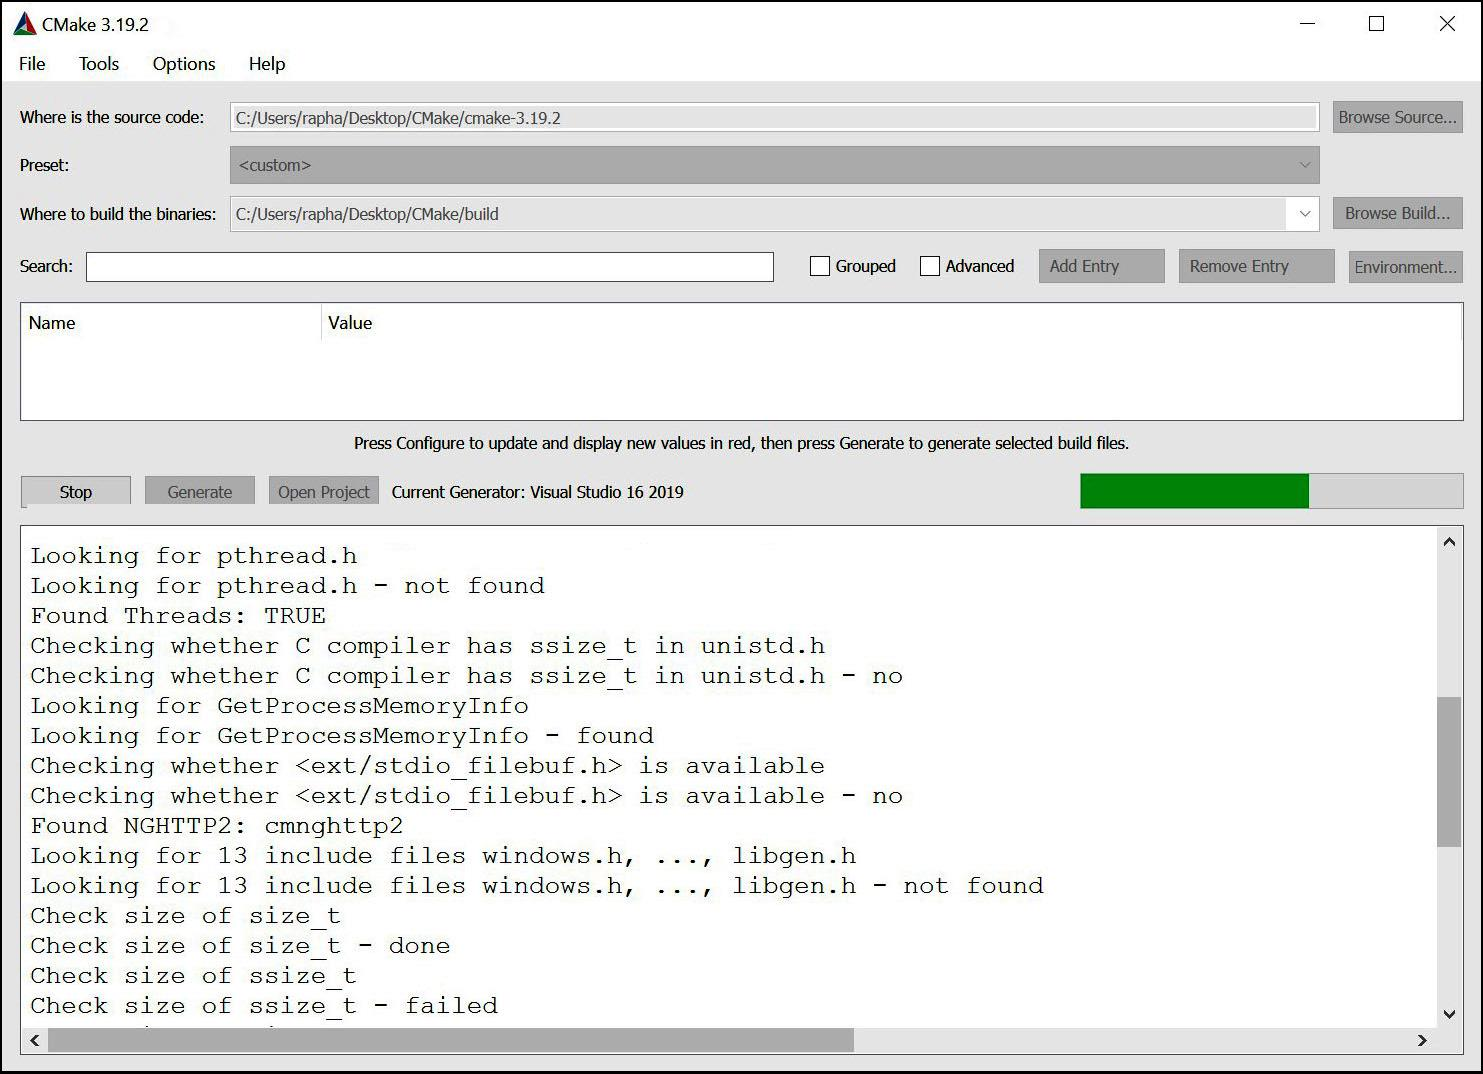
\includegraphics[width=0.9\textwidth]{content/1/chapter1/images/4.jpg}\\
图1.4  CMake GUI —— 使用Visual Studio 2019生成器构建系统的配置阶段
\end{center}

GUI应用程序对于用户来说是一个方便的工具,因为其中的选项相当有限。对于那些不熟悉命令行而更喜欢基于窗口的界面的人来说,它可能很有用。

\begin{tcolorbox}[colback=red!5!white,colframe=red!75!black,title=不推荐]
我会向终端用户推荐GUI,作为一名程序员,避免引入任何手册,阻止每次构建程序时都需要单击表单的步骤。这对于CI流水中的构建自动化尤其重要。这些工具需要无头软件,这样构建就可以在没有任何用户交互的情况下执行。
\end{tcolorbox}

\subsubsubsection{1.4.5\hspace{0.2cm}CCMake}

ccmake可执行文件是CMake面向类Unix平台的接口(它不适用于Windows)。它不是CMake包的一部分,所以用户必须单独安装。
 
Debian/Ubuntu系统的命令如下:
 
\begin{tcblisting}{commandshell={}}
$ sudo apt-get install cmake-curses-gui
\end{tcblisting}
 
注意,可以通过此GUI以交互方式指定项目配置设置。当程序运行时,终端底部会给出简短的说明:
 
\begin{tcblisting}{commandshell={}}
# CCMake命令的语法

ccmake [<options>]
ccmake {<path-to-source> | <path-to-existing-build>}
\end{tcblisting}
 
CCMake使用与cmake具有相同的选项集:
 
\begin{center}
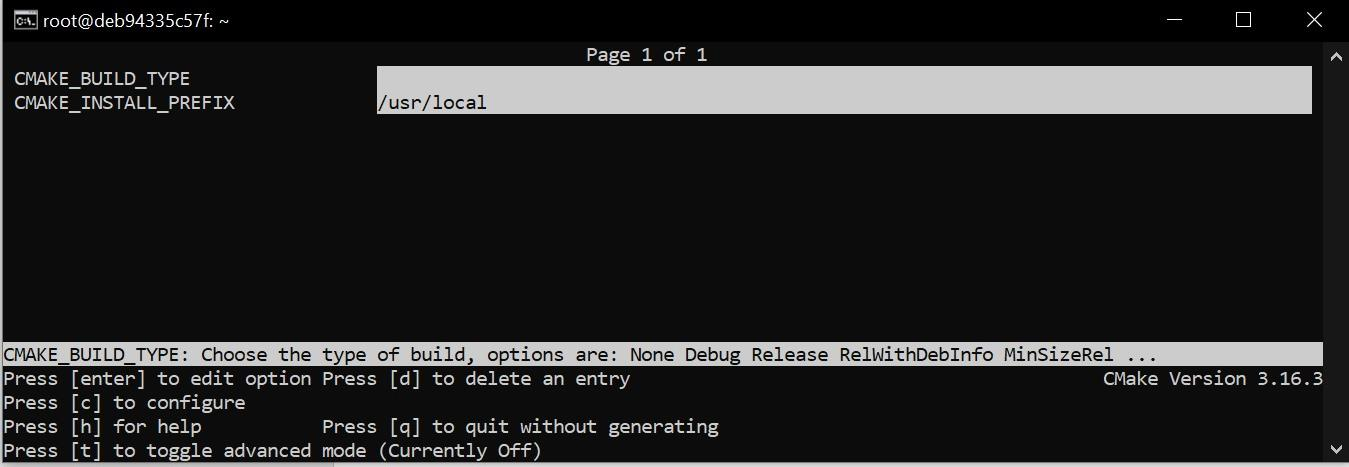
\includegraphics[width=0.9\textwidth]{content/1/chapter1/images/5.jpg}\\
图1.5  ccmake的配置阶段
\end{center}
 
与图形用户界面(GUI)一样,这种模式具有相当的局限性,仅供经验不足的用户使用。

以上就是对CMake命令行的基本介绍。接下来,来了解一下CMake项目的结构。
 
 
 
 
 
 
 
 
 
 
 
 
 
 
 
 